\section{Use case identification\label{sec:UseCaseDiscovery}}

\subsection{Criteria for use case identification}

In this Section, we identify use cases relevant to real-world applications~\cite{2023arXiv230613126S}.
In such identification, we will rely on the following criteria:

\begin{enumerate}
\item
Potential impact: selecting real-world use cases requires identifying research topics at the frontier of materials science and engineering that could benefit from the deployment of quantum computing for solving one or more of the discovery steps involved. Representative examples include semiconductor integration and processing, electronics, and optoelectronics applications. Also, materials use cases in carbon capture and storage, catalysis, energy storage, materials replacement, and recycling are being intensely researched, along with pharmaceutical and biochemical applications. In some cases, impact arises from insight into fundamental phenomena, while in other cases it comes from screening a large number of candidate materials and selecting the highest-performing candidate.
\item
Physical scale: typically, realistic materials use cases involve computational workflows consisting of various simulation steps with length and time scales covering more than 10 orders of magnitude. Therefore, predicting a material’s performance, from the molecular scale to the process scale, requires a broad range of computational methodologies including classical and quantum mechanical molecular dynamics simulations as well as the thermodynamic and bulk continuum models. Recently, artificial intelligence and machine-learning techniques have been added to the physics-based simulations toolkit for applications including generative materials design, high-throughput materials screening, and accelerated simulation.
\item
Complexity: application-guided and performance-oriented computational discovery work streams feature complex materials, where important phenomena occur in volumes often consisting of thousands of molecular building blocks with millions of atoms.  These are challenging to represent adequately in any computational simulation environment. A real-world discovery use case requires, therefore, the identification of a minimum representative materials volume for conducting the performance analysis. This representation can be as small as the active space within a molecule, a surface at which a physical or chemical process occurs, or as large as an entire composite wing of an airplane.
\end{enumerate}

In principle, quantum computing could be applied in each discovery step with the potential of enhancing computational accuracy, reducing computational time, or delivering any other improvement of the materials discovery outcome. For selecting the proper application of quantum computing in a real-world use case, it is however important to first identify and compare the difficulty of the classical and quantum simulation tasks and to ensure that proper data representations and algorithms can be developed for performing the discovery task on a quantum computing system. To that end, in our analysis of use cases, we will consider:

\begin{enumerate}
\item the relevance to real-world problems
\item the hardness of simulating the use case under consideration on classical computers
\item the hardness of simulating the use case under consideration on quantum computers (near-term and fault-tolerant)
\item the hardness of simulating quantum circuits involved in the previous point on quantum hardware and with classical simulators 
\item the possibility of using classical HPC and quantum computers in concert
\end{enumerate}

\subsection{Overview of use cases}

\begin{figure}
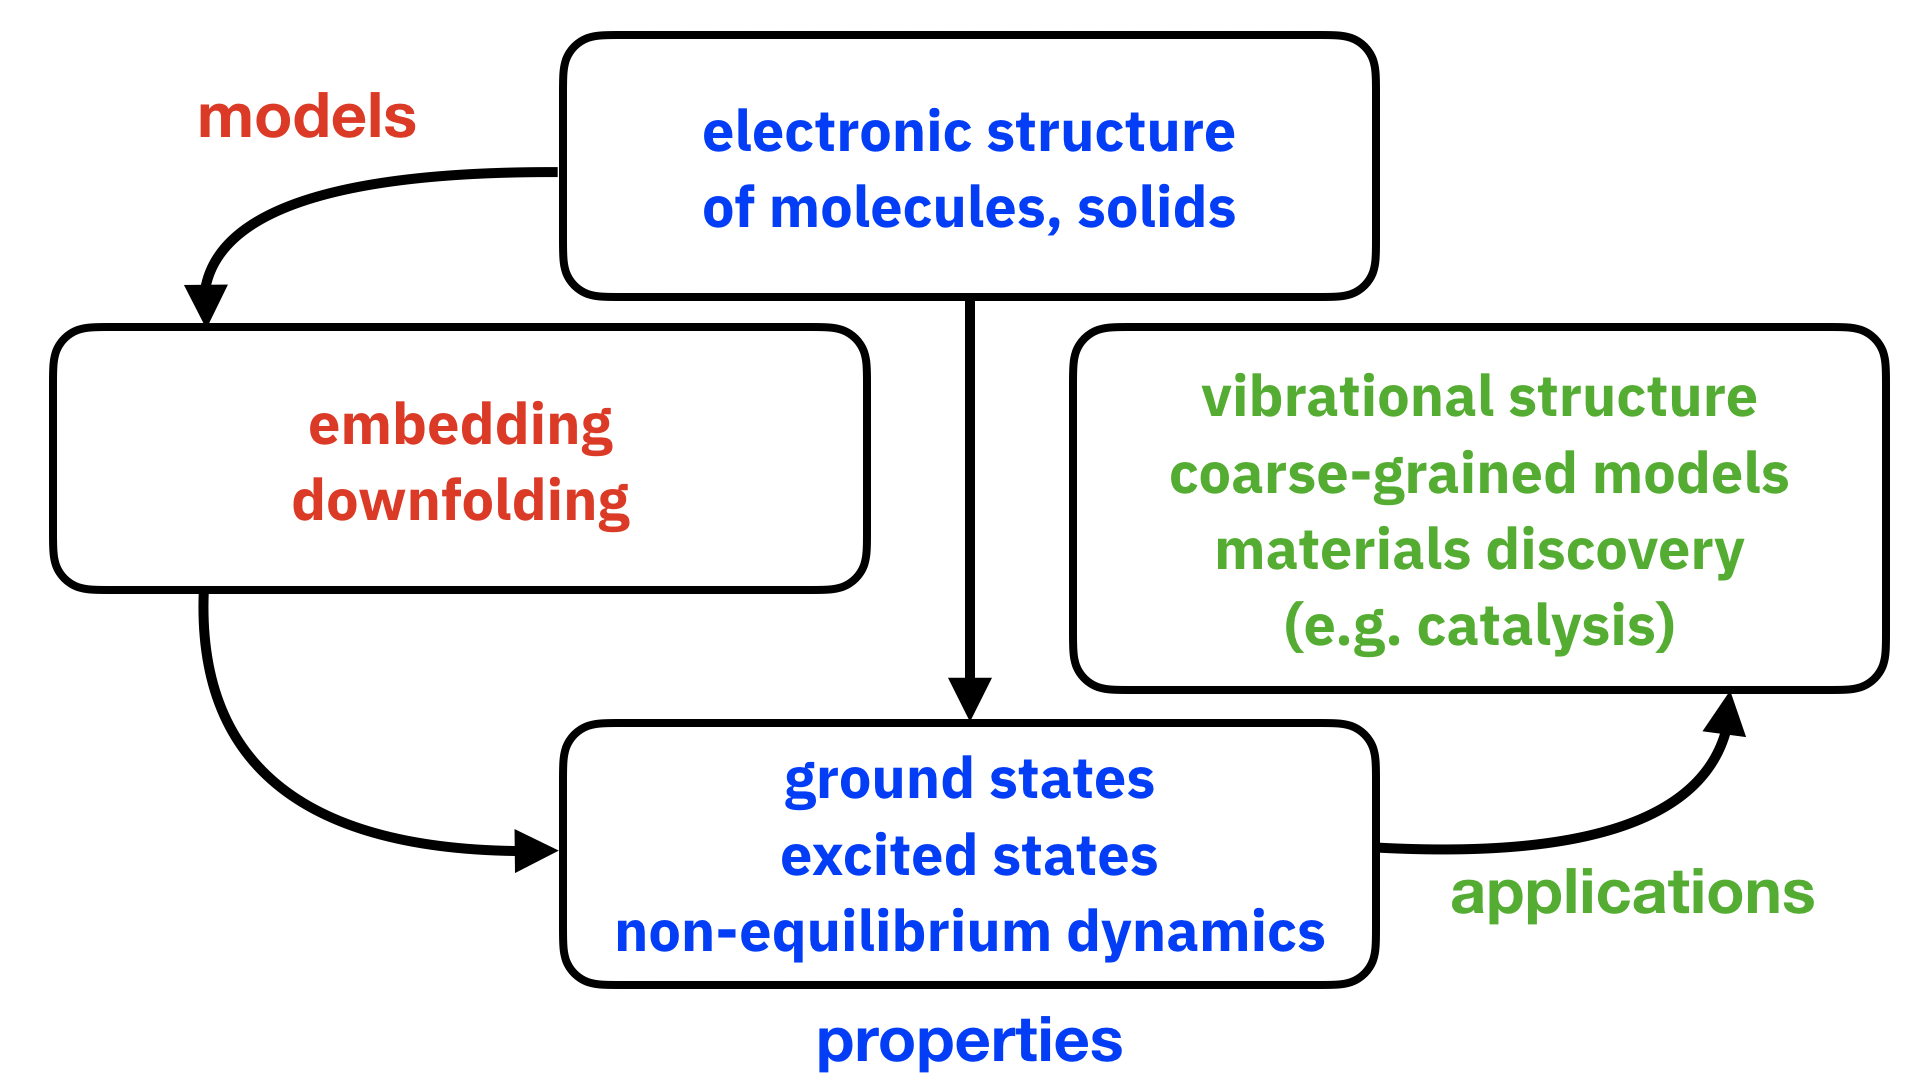
\includegraphics[width=\columnwidth]{groups/2._Use_case_discovery/map.png}
\caption{Schematics overview of use cases in materials discovery.  A central task of quantum theory is describing the properties of molecules and solids (blue). This goal can be achieved by solving for the electronic Schrodinger equation to compute e.g. ground-state, excited-states, and non-equilibrium dynamical properties (vertical arrow). Due to computational limitations, one can introduce approximations to the fundamental electronic structure problem, that reduce the size of the quantum problem within the existing computational budget (red).
Accurate solutions of the electronic Schrodinger equation are the starting point (green) for important applications in materials science, including vibrational structure calculations, coarse-grained models (e.g. corrosion, deformation), and materials discovery (e.g. catalysis, metamaterials).
}
\label{fig:map}
\end{figure}

A central task of quantum theory, in the fields of quantum condensed matter physics and quantum chemistry, consists of describing the properties of interacting atomic, molecular, amorphous, and crystalline systems. Apart from advancing our fundamental understanding of quantum mechanics, a generic solution to the quantum problem would allow progress in application fields ranging from materials discovery (better magnets, solar cells, catalysts, or qubit hardware) to drug design.

The required operation count and the number of quantum degrees of freedom required for the accurate ab initio description of such systems puts them far outside of the accessible regime on current or near-term quantum hardware, except for very small systems. These requirements were elucidated by many authors including Reiher et al \cite{reiher2017elucidating},Tubman et al \cite{2018arXiv180905523T}, Elfving et al \cite{elfving2020will} and Goings et al \cite{goings2022reliably}, who considered the application of quantum phase estimation to challenging instances of the electronic structure problem (respectively nitrogenase cofactor, chromium dimer, and cytochrome P450) on fault-tolerant devices.

It is therefore advantageous to consider approximations to the fundamental electronic structure problem that reduce the size of the quantum problem both in terms of qubit and operation requirements (see Figure~\ref{fig:map}, left).

Two complementary approaches are presently pursued. First, the embedding route identifies a set of strongly quantum parts of the problem (typically ``orbitals'' or ``sites''), extracts the relevant physics to an auxiliary quantum problem, and solves this problem using a quantum processor. The remainder of the system is then treated classically with polynomial scaling approximations. The exact limit is recovered by enlarging the embedding subspace or increasing the accuracy of the classical method.

Second, the model systems route approximates the original quantum system by a minimal set of appropriately chosen effective low-energy degrees of freedom. In this scheme, the exact limit is recovered in a ``bottom-up'' approach by gradually adding degrees of freedom until the original model is recovered. A typical example of this approach is given by the Heisenberg spin model, which (in the appropriate limit) captures the low-energy limit of the so-called t-J model, which itself is an approximation of the low-energy physics of the Hubbard model.

For both of these approximation approaches, simulation on quantum computers will become feasible much earlier than the simulation of the full quantum electronic structure problem. Realistic embedding approaches for materials typically result in compact but dense quantum problems (requiring many operations on few qubits), whereas model systems generally yield larger but sparse systems (requiring many qubits but fewer operations). The sparsity allows us to take advantage of devices with limited qubit connectivity with a reasonable operation count.

A central question concerns the physical observables under study. Traditional electronic structure mainly investigates ground states and their properties, such as the ``band structure'' or the ground-state energy as a function of nuclear coordinates. Out of these states, information about structure, vibrational modes, and mechanical properties is inferred.

However, experiments are performed at non-zero temperatures and, additionally, probe aspects of the excitation spectra. Photoemission spectroscopy, for instance, obtains the single-particle excitation spectrum and the gap size \cite{10.1063/5.0044060}. Nuclear magnetic resonance and magnetic neutron spectroscopy obtain nuclear spin excitations, and optical conductivity measurements probe two-particle excitations related to a current-current correlation function. Standard ground state methodology such as density functional theory (DFT) requires additional approximations to predict such observables. Famously the DFT ``band gap'' is not a reliable proxy for the gap in semiconductors \cite{bandgap,perdew1985density,cohen2012challenges}.
Quantum (or classical) computing methodologies that intrinsically contain excitation information present a valuable addition to our materials toolkit.

In many experimental setups, a weak external field (such as an incident light beam) probes the physics of the material under study. A central assumption is that this field leaves the material essentially unperturbed, such that linear response theory provides an appropriate description for its physics. However, once fields become strong, the system itself acquires an explicit time dependence which may often be modeled as a quench (an instantaneous change of the Hamiltonian such as a very short but very strong light pulse), a steady state (the time-evolution of a system in a translation-invariant long-time limit, such as a system with an applied voltage after initial transients have decayed), or a periodic drive (such as a continuous laser field).

While our classical toolkit for simulating ground-state physics is rather mature, the study of excitations within linear response is much more demanding and often requires high-performance computing resources. The study of time-dependent phenomena in real materials is still in its infancy. These science domains therefore offer promising application fields for future quantum computers. 

Reliable solutions to the electronic structure problem also allow us to define the nuclear Schrodinger equation, which in turn can be solved to determine molecular vibrations, and coarse-grained models, whose solution allows us to characterize complex phenomena including material stress, corrosion, and cracking (see Figure~\ref{fig:map}, right).

\subsection{Relevant use cases}

\subsubsection{Ground-state electronic structure}

One of the goals of electronic structure is to determine the ground and low-lying eigenstates of the Hamiltonian of a molecule, often within the Born-Oppenheimer approximation, i.e., for a fixed set of nuclear positions ${\bf{R}}$.
Determining the main features of the potential energy surface, i.e. the electronic energy as a function of nuclear positions $E({\bf{R}})$, is key to understanding chemical reactivity, reaction rates, and product distributions.
In particular, accurate estimation of reaction barrier heights (i.e. within $\sim 1$ kcal/mol from experiments) is important for many applications, such as catalyst development, battery electrode modeling, and manufacturing process design,
and a known challenge for electronic structure methods and in particular for DFT \cite{cohen2012challenges}.

As an example, in the design of manufacturing processes, the desired reaction(s) should dominate, e.g., have lower reaction barrier heights than undesired reactions.  One way to arrange this is through reactant selection, however, there may be many possible reactants.  Experimental screening to identify the best reactant candidates is often time, cost, and labor-intensive due to various factors.  Reactants may be expensive, hazardous, or rare.  Computational screening methods offer the possibility of screening candidate reactant barrier heights orders of magnitude faster, safer, and cheaper than experimental methods.  However, current state-of-the-art classical computational methods are often insufficiently accurate to compare reactant barrier heights.

\paragraph{Static and dynamic correlation}

Within electronic structure, wavefunctions are often classified as single-reference and multi-reference. In the former case, a single electronic configuration dominates the target wavefunction.
While the ground states of the majority of molecules have a single-reference character, one often encounters a multi-reference character in molecular excited states, at stretched bond geometries, in transition-metal chemistry, and in the presence of small HOMO-LUMO gap (e.g. large $\pi$-conjugated systems).

Single-reference problems can be accurately solved with various quantum chemistry methods for classical computers, from DFT methods (that can routinely treat $O(10^3)$ atoms~\cite{jones2015density})
to high-level wavefunction methods such as coupled-cluster theory (that can attain kcal/mol accuracy on systems of $O(10)$ atoms~\cite{sparta2014chemical}).
Extending quantum chemistry methods to multi-reference situations is an active and challenging research field where, notwithstanding steady progress, the accuracy attainable in molecules with more than a $O(1)$ atoms is significantly lower than in the single-reference case.

Important examples of multi-reference quantum-chemical problems are found in transition-metal chemistry~\cite{doi:10.1021/acs.jctc.9b00674,ciapprox-1}. Transition-metal oxides are an important class of materials that are used in catalysts, semiconductors, pigments, and many other applications.  Benchmarking studies of DFT for bond dissociation enthalpies of transition metal oxides and their cations demonstrate mean absolute errors of 30 kJ/mol (7 kcal/mol) or greater \cite{moltved2019performance}, identifying the energetics of reactions involving transition metals as a challenge for DFT \cite{moltved2019performance}. Examples of challenging instances of the electronic structure problem connected with transition-metal chemistry are:

\begin{enumerate}
\item Active sites of enzymes containing transition metals. These often involve multiple coupled transition metals, exemplified by the systems in Figure \ref{fig:fes}:
\begin{itemize}

\item the \ce{Fe2S2} and \ce{Fe4S4} clusters of ferredoxins \cite{sharma2014low}, where multi-reference character can be investigated in (30e,20o) and (36e,54o) active spaces respectively \cite{li2008github,li2017spin}

\item the iron-molybdenum cofactor (FeMo-cofactor) of nitrogenase, which catalyzes the 6-electron reduction of N$_2$ to ammonium in biological nitrogen fixation~\cite{noodleman2002insights,reiher2017elucidating}, and can be modeled by a (113e,76o) active space \cite{li2008github,li2019complexity}

\item the P-cluster of nitrogenase~\cite{li2019electronic} and oxygen-evolving complex of photosystem II \cite{cady2008functional,kurashige2013entangled}. In the context of nitrogenase, the hypothesized function of the P-cluster is to mediate electron transfer from the Fe-cluster to the FeMo-cofactor where nitrogen reduction takes place. The relevant states are the resting state \ce{P^N}, the one-electron oxidized state \ce{P^{1+}}, and the two-electron oxidized state \ce{P^{OX}}, which can be modeled by (114e,73o), (117e,75o) and (120e,77o) active spaces respectively.
\end{itemize}
Active sites of enzymes containing transition metals present highly complex multi-reference quantum chemistry problems motivated by biological applications.
Combined theoretical and experimental studies, primarily at the level of DFT, have illustrated many structural and electronic features of such active sites~\cite{siegbahn2009structures,lancaster2011x,batool2019magnetic}.
On the other hand, to interpret aspects of experimental spectroscopy, it is necessary to achieve a detailed understanding of the interplay between spin-coupling and delocalization between metals, which in turn requires accurate multi-reference quantum chemistry~\cite{sharma2014low,kurashige2013entangled,li2019electronic,chilkuri2019ligand,cao2018protonation}.
%
\item Nanocatalysts and surface catalysts containing transition metals. Simulating the mechanism of action of synthetic heterogeneous catalysts is challenging, as in the case of enzymes.
DFT predictions of quantities such as the adsorption energy of small molecules are unreliable~\cite{schimka2010accurate,capdevila2016performance}. 
While not all such problems are expected to be multi-reference in character, even the single-reference modeling of such chemistry, at a level significantly beyond DFT, is currently challenging or impossible.
In addition, multi-reference effects are expected to play a role in certain catalysts, such as transition metal oxides, or at intermediate geometries in reaction pathways~\cite{norskov2011density,schimka2010accurate,wodtke2016electronically,norskov2009towards}. 
\end{enumerate}

\begin{figure}
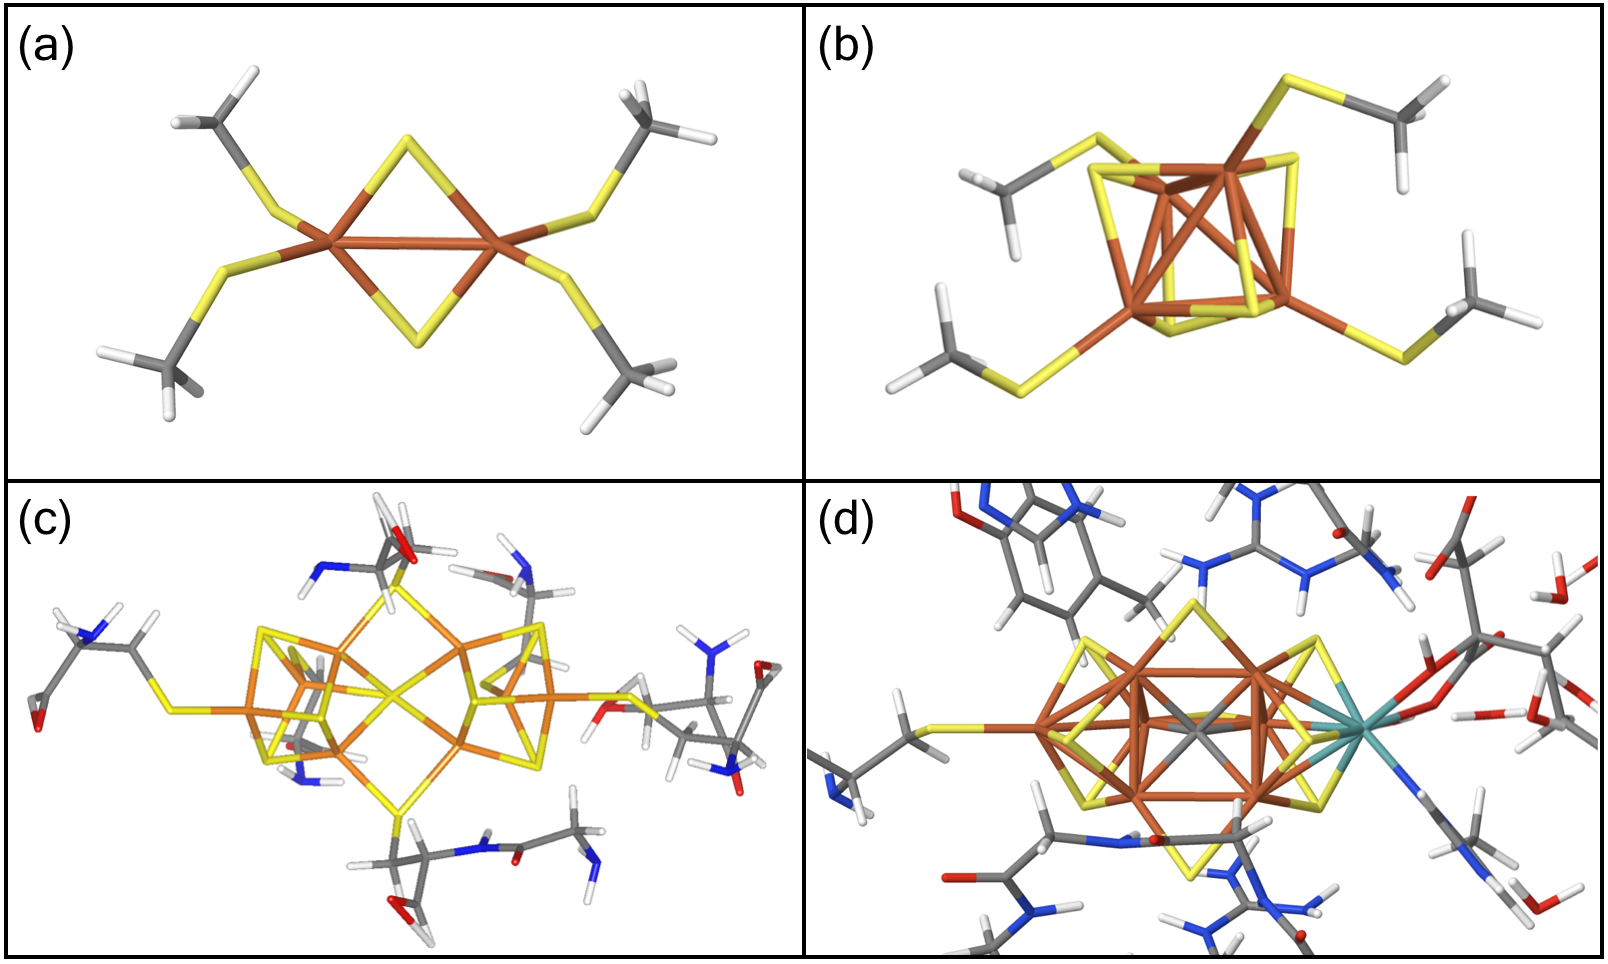
\includegraphics[width=\columnwidth]{groups/2._Use_case_discovery/fes.png}
\caption{The \ce{Fe2S2} (a) and \ce{Fe4S4} (b) clusters of ferredoxins, the P-cluster of nitrogenase in the resting state \ce{P^N} (c), and the FeMo-cofactor of nitrogenase (d). Orange, yellow, teal, red, blue, gray, and white sticks denote Fe, S, Mo, O, N, C, and H atoms respectively.}
\label{fig:fes}
\end{figure}

For all these systems, the basic quantum simulation problem is the computation of the ground-state (or low-energy eigenstate) of the electronic Hamiltonians, 
and the basic metric is whether quantum algorithms yield more accurate energies (for comparable computational resources) than their classical counterparts.
Proof-of-principle demonstrations can be carried out in the active spaces listed above.
However, to describe the actual chemistry of these systems, one should improve over active-space calculations by (i) treating larger numbers of electrons and orbitals, 
(ii) accounting for environmental, dynamical, and solvent effects, and (iii) accounting for dynamical electronic correlation.  While multi-reference problems are a known computational challenge,
even single-reference problems become hard to model classically when large numbers of electrons and orbitals are involved~\cite{vandevondele2012linear}.

\paragraph{Relativistic effects}

A discussion of the advantages and present challenges posed by hybrid quantum-classical approaches to electronic structure calculations begs mention of the treatment of relativistic effects.  
Accurate modeling of the ground and excited states of many molecules, such as atomic gold and uranium dimers, are examples of systems whose precise computational treatment requires the inclusion of relativistic effects in the Hamiltonian.  
Without this inclusion, a fundamental precision limit to quantum computation remains in place \cite{stetina2022simulating}.

\paragraph{Correlated electronic structure in solids}

There is some overlap in methods and ideas between the electronic structure problem in materials, e.g. crystalline solids, and quantum chemistry.
When electron-electron interactions are weak, the low-energy properties of a material can be described by computing the band structure using DFT. However, in some materials (called strongly correlated), the electron-electron interaction fundamentally changes the behavior and the effective non-interacting ansatz underpinning DFT is no longer appropriate. Typical examples are Mott insulators, which appear as conductors in band-structure theory but are insulating due to electron-electron interaction.
While Mott insulators are now well understood, many other phenomena in strongly correlated systems lack a justification in terms of an underlying microscopic mechanism and a quantitative and predictive theory of the associated physics.
Some important examples include:

\begin{itemize}
\item \textit{High-temperature superconductivity}. The mechanism driving superconductivity is not yet fully elucidated. Two regimes close to superconductivity, the {pseudogap} and {strange-metal} phase remain elusive~\cite{keimer2015quantum}. The nature and relation to the superconducting phase of both are not understood. The strange-metal phase features behavior inconsistent with a simple weakly interacting metal even at high energies, hence the name of ``non-Fermi liquid phase'', and has motivated a whole area of research on exotic metallic systems~\cite{lee2018recent}. On the other hand, the pseudogap phase features several competing ordering tendencies~\cite{fradkin2015intertwined}, which are very challenging to resolve in numerical methods, because most methods naturally favor a particular ordering pattern, so discriminating physical effects from method biases is very difficult.
\item \textit{Frustrated spin systems} realize a host of high non-trivial phases, in particular topological and gapless spin liquids~\cite{balents2010spin}. They have historically been the test bed for computational methods such as tensor networks and variational methods and, as such, appear as good test cases for quantum simulations.
\end{itemize}

\subsubsection{Embedding}
\label{embedding_sec}

As seen in the previous Section, solving the electronic structure problem in situations that are relevant to real-world applications, e.g. catalysis, requires significant quantum resources.
That example illustrates how the goals of relevance to real-world applications and ease of execution on quantum devices are in conflict.
However, there are two ways of making feasible progress toward the solution of challenging instances of the electronic structure problem: quantum embedding theories and effective low-energy models. 
These are not only useful steps toward the electronic structure problem, but also very compelling applications for current and near-term devices. Examples and applications are described in the remainder of this and following Sections.

The idea of quantum embedding theories stems from the fact that in chemistry, physics, and materials science, phenomena of interest often take place within a small region, motivating the separation of the whole system into a so-called active space surrounded by a host environment. The electronic structure problem is solved separately for the environment at a low level of theory and for the active space at a higher, i.e., more accurate and more expensive, level of theory. As an active space only accounts for a small portion of the whole system with a greatly reduced Hilbert space, simulating it using quantum chemistry methods becomes feasible on quantum computers and emulators. Examples of active spaces include point defects in semiconductors and insulators and active sites of catalysts at interfaces or on surfaces.

Various quantum embedding theories have been proposed, categorized by the level of theory used to describe different parts of the system.
\begin{itemize}
\item Density-based embedding theories define an active space in real space and partition the density of the system into the active space and the environment. The latter is described at the DFT level, and the former is described either using DFT with a higher-level exchange-correlation functional (DFT-in-DFT) or with wavefunction-based quantum chemistry methods (WF-in-DFT).
%
\item Density matrix embedding theories (DMET)~\cite{knizia_density_2012,knizia_density_2013,wouters_practical_2016,pham_can_2018,hermes_multiconfigurational_2019,pham_periodic_2020,cui_efficient_2020,lau_regional_2021,cui_systematic_2022,mitra_density_2023}, as introduced previously, also define an active space in real space. The active space is treated at a higher level of theory. The interaction with the environment is accounted for through a set of bath orbitals obtained from a calculation of the full system at a lower level of theory, with an additional one-body term that ensures the density matrices at both levels of theory coincide.
%
\item Embedding theories based on Green's function define an active space by a set of single-particle electronic states. The non-local, frequency-dependent self-energy of the active space is expressed as a sum of terms evaluated at high and low levels of theory, with an additional term to remove the double counting. Examples of such theories include dynamical mean-field theory embedding (DMFT+DFT~\cite{anisimov_first-principles_1997,lichtenstein_ab_1998} or DMFT+GW~\cite{sun_extended_2002,biermann_first-principles_2003,biermann_dynamical_2014,boehnke_when_2016,choi_first-principles_2016,nilsson_multitier_2017}), self-energy embedding theory (SEET)~\cite{lan_generalized_2017,zgid_finite_2017,rusakov_self-energy_2019}, and quantum defect embedding theory (QDET)~\cite{ma_first-principles_2020,ma_quantum_2020,ma_quantum_2021,sheng_greens_2022}. They mainly differ in the choice of the high-level and low-level theories and the partitioning of the total self-energy into the active space and the environment.
\end{itemize}

In practice, a quantum embedding calculation typically starts with a low-level calculation of the full system, the results of which are subsequently employed to determine parameters of the many-body effective Hamiltonian of the active space. In QDET, for example, the effective Hamiltonian comprises a one-body term and a two-body term. In the one-body term, an exact double counting correction has been derived for the case where G$_0$W$_0$ is the low-level theory. In the two-body term, the effect of the environment is incorporated through an effective screening. The QDET Hamiltonian can be computed without any explicit summation over empty states, enabling its application to large systems. Leveraging GPU-accelerated classical supercomputers, it is feasible to simulate systems consisting of over a thousand atoms and active spaces consisting of over a hundred orbitals. The effective Hamiltonian, written in second quantization, can be diagonalized on classical computers using FCI, or on quantum computers~\cite{ma_quantum_2020,rungger_dynamical_2020,keen_quantum-classical_2020,kawashima_optimizing_2021,yao_gutzwiller_2021,tilly_reduced_2021,vorwerk_quantum_2022,huang_simulating_2022,huang_quantum_2023} by mapping it to qubits and quantum gates and finding its lowest eigenstates using a suitable quantum eigensolver.
%
Challenges remain in facilitating the communication of data from classical (super)computers to quantum computers, accommodating the effective Hamiltonian with the available number of gates and circuit depth, and mitigating noises present on near-term computers which may lead to unphysical results. Intriguingly, quantum computers themselves are employed to investigate the properties of spin defects in solids. These defects hold promise as prospective candidates for the implementation of improved quantum computers, thus forming a positive feedback loop at the intersection of computational materials science and quantum computing.


Additionally, CAS-DMET and NEVPT2-DMET described before have been effectively used to examine the adsorption and emission spectra of the negatively charged nitrogen-vacancy (NV$^{-1}$) and the neutral silicon vacancy (SiV$^{0}$) defects in diamond, as well as the neutral oxygen vacancy (OV$^{0}$) defect in both bulk and surface magnesium oxide, as reported in recent literature. \cite{mitra2021excited,haldar2023local,Verma2023} In particular, for the NV$^{-1}$ defect in diamond, NEVPT2-DMET with a significantly reduced embedding space and a complete active space (CAS) configuration of 10 electrons in 9 orbitals (denoted as 10e, 9o) accurately predicts a triplet-triplet excitation energy of 2.31 eV. This is in close agreement with the experimentally observed value of 2.18 eV. Additionally, it predicts an optically inactive singlet-singlet transition at 1.02 eV, closely approximating the experimental value of 1.26 eV. For the neutral OV$^{0}$ defect in MgO bulk, NEVPT2-DMET, with a CAS configuration of 2e, 5o, estimates the excitation energy to be 5.24 eV, aligning well with the experimental absorption maximum of 5.03 eV. Studies of the optically allowed $S_0\rightarrow S_1$ transition for the OV$^{0}$ defect on the MgO surface have also been conducted using CAS-DMET, NEVPT2-DMET, and DME-PDFT methods. However, varying experimental results ranging from 1-5 eV have been reported, which makes direct comparison difficult. Using MP2 and CCSD solvers for the DMET embedding subspace, the adsorption energies for CO on MgO have been calculated using the largest embedding subspaces, and these have been found to be within 1.2 kcal/mol of the non-embedding reference values. \cite{Mitra2022} So far, the LASUCC and LASSI methods have primarily been tested on strongly correlated molecular systems and has been utilized to study the dissociation of (H$_2$)$_2$ into two H$_2$ molecules, the dissociation of the two double bonds in trans-butadiene, and the $J$-coupling in tris-(\(\mu\)-hydroxo)-bridged chromium compound model~\cite{Pandharkar2022,Otten2022}. The accuracy of these studies has been confirmed through excellent agreement with the results from corresponding CASCI calculations performed using LAS orbitals.

\subsubsection{Model systems}

Low-energy models introduce an effective Hamiltonian describing the low-energy degrees of freedom of a quantum system. The effective Hamiltonian is then solved for the ground- and low-energy excited states.
How to propose a low-energy effective Hamiltonian, and how to propose reliable and precise parameters for that Hamiltonian, are important questions that affect the predictive power of that model for real-world applications.
On the other hand, accurate solutions of a given model allow us to capture trends in physical properties as the free parameters of the model vary (e.g. temperature, interaction strength, number of electrons).
Therefore, the value of a model as it relates to real-world application lies both in its definition and in its computational solution: the physical properties predicted by a model should be equally robust to perturbations in model parameters and solutions of the Schrödinger equation, for robust inferences about the physical properties of a real system to be drawn from the use of effective low-energy models.

The dominant effective model for quantum particles in materials is band structure, and for metals, Fermi liquid theory. However, a major challenge is how this paradigm should be altered when it is no longer a good description of the physical system. Examples of these include the high-T$_c$ cuprates and other transition-metal compounds like spin liquids, which do not appear to be well-described by these simple effective Hamiltonians. For these systems, many models have been proposed, such as the Emery and Heisenberg reviewed below. While these models have been extensively studied analytically and numerically, and have significantly enhanced our understanding of the physics of correlated electrons, their effectiveness for describing a real complex system of interest is often unclear. At the same time, more complex effective models can be commensurately more difficult to solve, so one would like to also find an accurate effective model that is computationally tractable.
Very importantly, most such models feature free parameters that need to be given precise values to be of relevance to the physics of high-T$_c$ cuprates and spin liquids. These parameters are often assigned starting from experimental data and/or classical electronic structure simulations, leading to both biases and uncertainties.

To address the need for a link between ab initio electron-level models and larger-scale models, downfolding has most commonly been carried out using approaches based on DFT. The effective one-particle hopping terms are obtained by projecting the DFT bands onto localized Wannier functions \cite{pavarini2001band}. The interactions are then estimated based on certain models of screening of the Coulomb interactions, e.g., constrained DFT, and Random Phase Approximations (RPA). Since the effects of interactions between the orbitals of interest have already been accounted for by DFT, a double-counting correction is required to obtain the final downfolded Hamiltonian. The approach has been developed and widely applied \cite{aryasetiawan2004frequency,jeschke2013first,haule2015exact} but remains an active area of research \cite{haule2015exact}. 
There are other downfolding approaches that include the traditional L\"{o}wdin method, coupled with a stochastic approach  \cite{ten2013stochastic,zhou2010construction}, and the related method of canonical transformations  \cite{white2002numerical,yanai2006canonical}. While they have many advantages, it is typically not possible to know if a given model ansatz was a good guess or not, and it is very rare for a technique to provide an estimate of the quality of the resultant model.

In the remainder of this Section, we review some important model systems, namely spin Hamiltonians and lattice models of correlated electrons. While the relationship between these models and real materials is very delicate, both due to the choice of the effective Hamiltonian and its parameterization, studying computationally the phase diagram of these models as a function of their free parameters can reveal trends and phase transitions that are relevant for the physics of real materials. Furthermore, it constitutes a promising research area for simulations on current and near-term quantum devices.

\paragraph{Spin Hamiltonians}

Spin Hamiltonians are frequently used to model the magnetic properties of materials as well as other systems where there is local correlation or frustration. Consider a lattice with $n$ sites occupied by spin-$s$ particles that are allowed to interact with each other.
In such a lattice, there is an allowed number of $2s+1$ microstates at each lattice site, giving a total of $(2s+1)^n$ spin configurations for a lattice with $n$ sites. 
At an infinitely high temperature, spins point randomly in all directions, agitated by thermal motion. 
On the other hand, as the temperature approaches $T=0K$, in many situations spins display the tendency to become part of a long-range magnetically ordered state under the effect of the interaction between them. The two extreme limits are antiferromagnetic order, where adjacent spins point in opposite directions, and ferromagnetic order, where all spins point in the same direction.
If we consider paramagnetism (namely the absence of magnetic order in the absence of an externally applied magnetic field) as analogous to an ideal gas (where particles interact weakly with each other), and magnetic order as analogous to a solid (where particles form a static and regularly repeating lattice), it is natural to inquire if there exists an analogous liquid of spins.

Spin liquids \cite{savary2016quantum,zhou2017quantum,chamorro2020chemistry,sears2017phase,PhysRevA.106.022434,li2023benchmarking} are exotic materials where spins do not order at any finite temperature but interact strongly with each other, unlike in a paramagnet where spins are weakly coupled to each other.
Normally, strong spin interactions result in a single spin configuration (or a small subset thereof) having lower energy than the others, thereby driving magnetic order.  In a spin liquid, interactions conspire to make all spin configurations (or a large subset thereof) nearly equivalent in energy, thereby evading magnetic order.
In a spin liquid state, the ground state consists of a superposition of spin configurations that is not dominated by a single configuration (or a small subset thereof). A spin liquid thus does not possess magnetic order, as individual spins fluctuate, but possesses strong entanglement in the ground state, so that spins are not randomly mutually oriented.

The key ingredient to obtain a ground state that is a superposition of a large number of spin configurations is to have strong interaction between neighboring spins and have a large number of configurations with near-identical energies, i.e. to frustrate the spins. This often arises due to the underlying geometric frustration of the lattice in which spins sit and/or the nature of the interaction between spins. Furthermore, particles with higher spin $s$ tend to show more classical behavior as opposed to quantum behavior, because the energy barrier between different microstates scales as $s^2$, which strongly suppresses quantum fluctuations. Therefore, a spin as low as possible, e.g. $s=1/2$, greatly favors spin liquid behavior.

\begin{figure}[htbp]
\centering
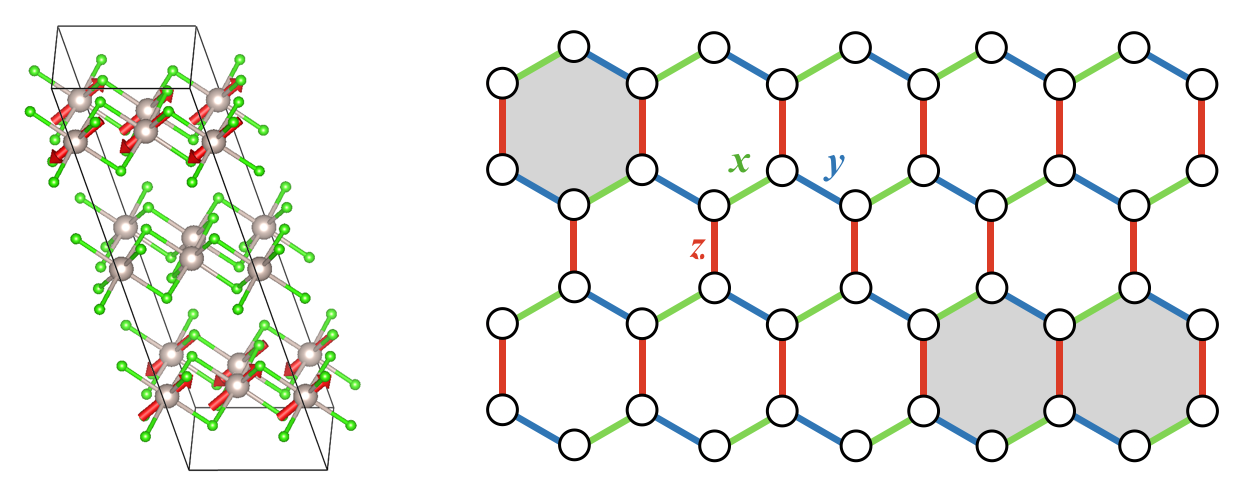
\includegraphics[width=\columnwidth]{groups/2._Use_case_discovery/spins.png}
\caption{Left: crystal structure of $\alpha$-RuCl$_3$, illustrating the van der Walls gap between the RuCl$_6$ honeycomb layers (with Ru/Cl atoms represented as gray/green circles) and magnetic Ru$^{3+}$ ions aligned as in the zigzag phase (red arrows). Right: schematic representation of the two-dimensional Heisenberg-Kitaev model with spins represented as white circles and $x/y/z$ bonds as green/blue/red links respectively. Quantum simulations to date have focused on 1 and 2 hexagons, corresponding to 6 and 10 spins respectively \cite{tazhigulov2022simulating}.}
\label{fig:rucl3}
\end{figure}

A concrete example of a material of interest as a proximate spin liquid \cite{chamorro2020chemistry} is ruthenium trichloride, $\alpha$-RuCl$_3$ (see Fig.~\ref{fig:rucl3}). This transition metal halide has a crystal structure made up of stacked honeycomb layers of edge-sharing RuCl$_6$ octahedra. Plumb et al \cite{plumb2014alpha} found that spin-orbit coupling in this material is substantial, leading to a $j=1/2$ description of the Ru$^{3+}$ valence electrons. 
Since this material is built up with edge-sharing RuCl$_6$ octahedra, it is believed \cite{kitaev2006anyons,jackeli2009mott} that its low-energy excitations are parametrized by the Kitaev-Heisenberg Hamiltonian
\begin{equation}
H_{kh} = \sum_{\langle ij \rangle_\gamma} J \vec S_i \cdot \vec S_j + K S_{i \gamma} S_{j \gamma} \;,
\end{equation}
where $\langle ij \rangle_\gamma$ denotes summation over the bonds $\gamma \in \{x,y,z\}$. This feature makes $\alpha$-RuCl$_3$ a material of great interest in the ongoing search for a Kitaev spin-liquid ground state \cite{koitzsch2016j,nasu2016fermionic,banerjee2016proximate}. Although $\alpha$-RuCl$_3$ orders magnetically at low temperature with zigzag magnetic order \cite{banerjee2016proximate,sears2015magnetic}, this material has shown some signatures of spin-liquid physics, such as a broad continuum of magnetic excitations identified in both Raman scattering \cite{sandilands2015scattering} and inelastic neutron scattering measurements \cite{banerjee2016proximate}.
Therefore, the degree of similarity to the Kitaev model, as well as the interpretation of spectroscopic and thermal measurements in terms of modifications to the Kitaev model, is currently intensely debated. We remark that, in the literature \cite{maksimov2020rethinking}, the Kitaev-Heisenberg Hamiltonian is augmented by additional couplings, 
\begin{equation}
\begin{split}
H &= H_{kh} + \sum_{\langle ij \rangle_\gamma} \Gamma ( S_{i\alpha} S_{j\beta} + S_{i\beta} S_{j\alpha} ) \\
&+ \sum_{\langle ij \rangle_\gamma} \Gamma^\prime ( S_{i\gamma} S_{j\alpha} + S_{i\gamma} S_{j\beta} + S_{i\alpha} S_{j\gamma} + S_{i\beta} S_{j\gamma} )  \;,
\end{split}
\end{equation}
with $\{\alpha,\beta,\gamma\} = \{x,y,z\} , \{z,x,y\}, \{y,z,x\}$ for $\gamma = z,y,x$ respectively. Several parameter configurations have been proposed to describe the Hamiltonian $H$, ranging from first-principle methods \cite{yadav2016kitaev,maksimov2020rethinking} to phenomenological analyses \cite{banerjee2016proximate,maksimov2020rethinking}. Recent literature has focused on $J = -1.53$, $K= -24.4$, $\Gamma = 5.25$, $\Gamma^\prime=-0.95$ \cite{tazhigulov2022simulating}. The coupling that is believed to be the leading one is the (negative) Kitaev term $K<0$. The off-diagonal exchange term $\Gamma>0$ is also believed to be significant, while the ferromagnetic exchange $J$ is believed to be subleading \cite{winter2017models}.
However, it should be noted that the parameters of $H$ vary quite significantly between the studies \cite{winter2016challenges,maksimov2020rethinking}. The exactly solvable Kitaev model corresponds to $J=\Gamma=\Gamma^\prime=0$, and it is argued that, in the parameter regime of $\alpha$-RuCl$_3$, both the excitations and the heat capacity show echoes of the two kinds of Majorana fermions that exist at the solvable point \cite{gohlke2017dynamics,laurell2020dynamical}.

The combination of rich physical behavior and challenging ground- and thermal-state preparation makes quantum spin liquid models like the Kitaev-Heisenberg Hamiltonian approximating $\alpha$-RuCl$_3$ interesting and challenging problems for classical and quantum simulations. The presence of $2$-local spin-$1/2$ Hamiltonians makes them compelling targets for simulations on quantum devices, focused on the calculation of specific heats and dynamical structure factors relevant to understanding the low-energy excitation spectrum of the Hamiltonian.

\paragraph{Lattice models}

A central feature of correlated electron materials is the competition between different inhomogeneous orders. Important examples are metal-insulator \cite{imada1998metal}, paramagnet-ferromagnet \cite{spaldin2010magnetic}, and conductor-superconductor phase transitions \cite{orenstein2000advances,dagotto1994correlated}.
Lattice models of correlated electrons serve as the canonical microscopic physical models for the computational description of such competition phenomena in materials.
A paradigmatic example of a fermionic lattice model is the one-band Hubbard model \cite{hubbard1964electron,kanamori1963electron,gutzwiller1963effect,arovas2022hubbard},
\begin{equation}
\label{eq:hubbard}
\hat{H} = -t \sum_{\langle ij \rangle \sigma} ( \hat{a}^\dagger_{i\sigma} \hat{a}_{j\sigma} + \mathrm{h.c.} ) + U \sum_i \hat{n}_{i \uparrow} \hat{n}_{i \downarrow} \;.
\end{equation}
In Eq.~\eqref{eq:hubbard} where $\hat{a}/\hat{a}^\dagger$ denote the usual fermion annihilation/creation operators, $\hat{n} = \hat{a}^\dagger\hat{a}$ is the number operator, $t$ and $U$ are the kinetic and repulsion energies,
and $\langle ij \rangle$ denote summation over nearest neighbors sites $ij$ on a lattice (e.g. the 2D square lattice).
The Hubbard model is one of the simplest models of interacting fermions, but despite its simplicity, it exhibits a wide range of correlated electron behavior including interaction-driven metal-insulator transitions, superconductivity, and magnetism. 
The precise behavior depends delicately on parameters, creating an interesting challenge for theory and computation.
Exact solutions are available for one-dimensional \cite{lieb1968absence} and infinite-dimensional cases \cite{metzner1989correlated}. 
High-temperature series expansions provide numerically exact results but only for temperatures too high to be relevant for physically interesting situations \cite{oitmaa2006series}. 
In general dimensions at relevant temperatures, only approximate numerical solutions are available, including wavefunction-based, diagrammatic, and embedding methods \cite{leblanc2015solutions}.
These numerical methods have been steadily developed and carefully benchmarked \cite{leblanc2015solutions,zheng2017stripe}, providing illuminating insights into the physics of this model.

\begin{figure}[h!]
\centering
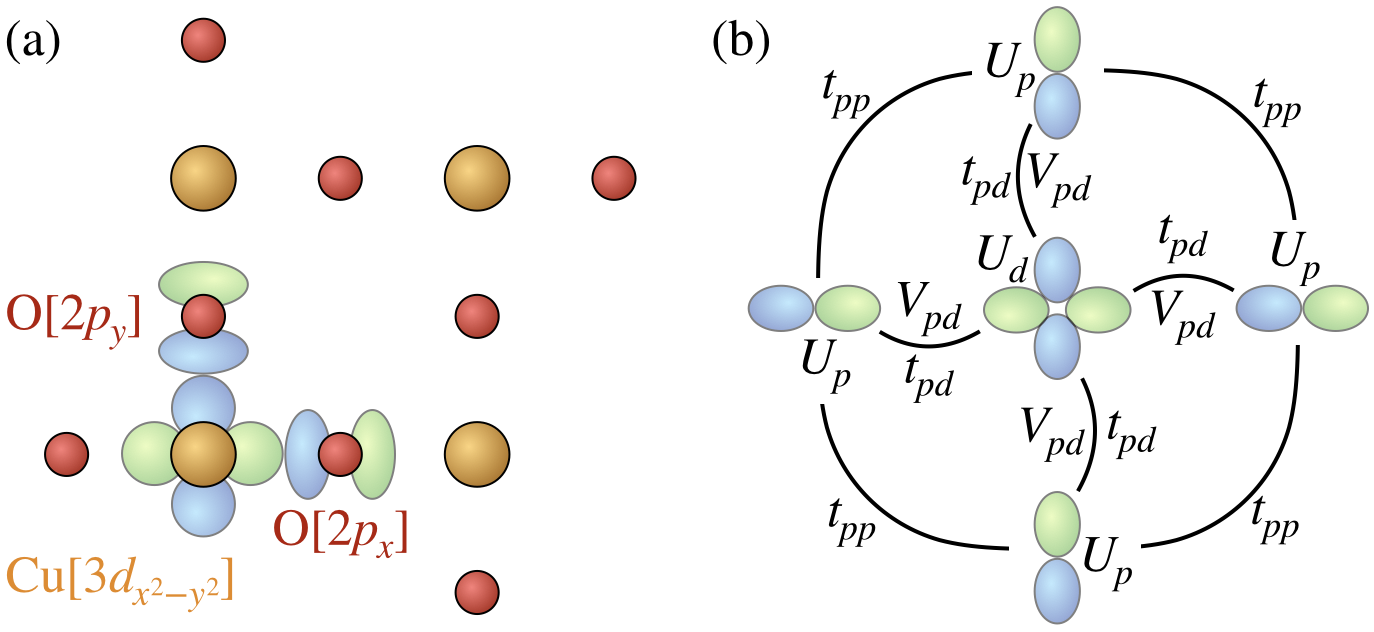
\includegraphics[width=\columnwidth]{groups/2._Use_case_discovery/lattice.png}
\caption{(a) schematic view of a [CuO$_2]_4$ cell in a cuprate CuO$_2$ plane. Cu/O atoms are represented with orange/red circles and orbitals by blue and green contour plots (blue/green for positive/negative values). (b) definition of the three-band Hubbard model parameters (the curve connectors represent the kinetic energy coefficients).
}
\label{fig:lattice}
\end{figure}

One concrete example of a fermionic lattice model that can be connected to a technological application is the three-band Hubbard model in two dimensions, also known as the Emery model \cite{emery1987theory}. 
This model is generally believed to contain the essential properties of high-T$_c$ cuprate superconductors that arise from the interplay between the copper $d_{x^2-y^2}$ and oxygen $p_{x,y}$ orbitals in the CuO$_2$ layers (see Figure \ref{fig:lattice}). It is defined, in the so-called ``phase representation'', by the Hamiltonian
\begin{equation}
\label{eq:emery}
\begin{split}
\hat{H} &= 
t_{pd} \sum_{\langle ij \rangle \sigma} (\hat{d}^\dagger_{i\sigma} \hat{p}_{j\sigma} + \mathrm{h.c.} )
+ t_{pp} \sum_{\langle ij \rangle \sigma} (\hat{p}^\dagger_{i\sigma} \hat{p}_{j\sigma} + \mathrm{h.c.} ) \\
&- \Delta_{pd} \sum_{i\sigma} \hat{n}^d_{i \sigma} \\
&+ U_d \sum_i \hat{n}^d_{i\uparrow} \hat{n}^d_{i\downarrow} 
+ U_p \sum_i \hat{n}^p_{i\uparrow} \hat{n}^p_{i\downarrow} 
+ V_{pd}  \sum_{\langle ij \rangle \sigma \tau}  \hat{n}^p_{i\sigma} \hat{n}^p_{j\tau} \, \\
\end{split}
\end{equation}
where $\langle \rangle$ denotes nearest neighbors, $d^{(\dagger)}_{i\sigma}/p^{(\dagger)}_{i\sigma}$ destroys (creates) a hole with spin $\sigma$ on the Cu[3d]/O[2p] orbital, $\hat{n}^d_{i\sigma}/\hat{n}^p_{i\sigma}$ is the number of holes on a Cu[3d]/O[2p] orbital with spin $\sigma$, and the charge transfer gap $\Delta_{pd}$ is defined as the difference between the O[2p] and Cu[3d] orbital energies.

On classical computers, the Emery model has been investigated with several numerical methods, including direct simulations of lattices by exact diagonalization of up to 24 sites \cite{greiter2007no}, 
quantum Monte Carlo and density matrix renormalization group (DMRG) of 80 and 144 sites \cite{huang2017numerical,vitali2019metal}, and embedding methods like density matrix embedding theory with 12 sites \cite{cui2020ground}.
These simulations have been primarily directed at simulating ground-state spin-spin, and $d$-wave correlation functions, to establish e.g. the presence of stripe or $d$-wave superconducting order \cite{greiter2007no,huang2017numerical,vitali2019metal,cui2020ground}.

Due to the complexity of the model, unlike in the one-band case, a consensus on much of the physics has yet to be reached, 
providing an opportunity for high-accuracy quantum computing algorithms to elucidate the properties of high-T$_c$ cuprate superconductors by simulating lattices of O(100) sites.

The Emery model is often simplified considering a one-band Hubbard model. While much of the physics of high-T$_c$ cuprate superconductors,
e.g. $d$-wave pairing, density waves, pseudogap phase, stripe order, is described by the one-band Hubbard model Hamiltonian,  there are still important reasons to go beyond the one-band picture to study the original three-band model directly. For instance, (a) some important physics may be lost in the reduction to the one-band approximation (such as a role for the oxygen degrees of freedom in the pseudogap phase \cite{fauque2006magnetic}), (b) near degeneracies of competing states seen in the one-band case \cite{zheng2017stripe} may be resolved with the additional degrees of freedom of the three-band model, and (c) the three-band model retains the atomic structure of the CuO$_2$ layer and thus has a direct link to the structure of real materials as well as experimental measurements of orders at the atomic scale \cite{hybertsen1989calculation,martin1996electronic,hanke20103}.

\subsection{Excited states}

Many experiments on condensed-matter systems probe dynamical properties, rather than equilibrium properties.
For example, material properties are often explored through scattering experiments, such as neutron and photon scattering or angle-resolved photoemission spectroscopy (ARPES)~\cite{Damascelli_2004}, 
which probe the structure factor and spectral function respectively~\cite{10.1063/1.5114818,2023arXiv231004333W}.
In these experiments, a system is initialized at equilibrium at inverse temperature $\beta$ under a Hamiltonian $\hat{H}$, and a time-dependent perturbation $\hat{V}(t)$ is applied. The response of the system is characterized by linear response theory, computing frequency-dependent correlation functions of the form
\begin{equation}
\label{eq:cabw}
C_{AB}(\omega) = \int_{-\infty}^{\infty} \frac{dt}{2\pi} \, e^{i\omega t} \, \mbox{Tr}[ \hat{\rho}(\beta) e^{it \hat{H}} \hat{A} e^{-it \hat{H}} \hat{B} ] \;.
\end{equation}
where $\hat{A},\hat{B}$ are suitable operators, e.g. components of the dipole moment operator and density operators at two different spatial points in UV/visible light and neutron scattering experiments respectively.
It should be noted that $C_{AB}(\omega)$ can be computed knowing the eigenpairs of the unperturbed Hamiltonian $\hat{H}$ and/or its time evolution operator $e^{-it \hat{H}}$.
In other words, by virtue of the linear response approximation, the perturbation $\hat{V}(t)$ does not appear in the function $C_{AB}(\omega)$.

Going beyond spectral properties, the {non-equilibrium real-time dynamics} of quantum systems have increasingly come into focus, both because of experiments that can probe quantum dynamics at atomic scales, 
{and because of fundamental interest in studying the equilibration of quantum systems, which serves as a bridge between the theories of quantum mechanics and statistical mechanics}. 
Experimental setups now exist that can probe ultra-fast dynamics in materials including, for example, free-electron lasers~\cite{patterson2010coherent,weathersby2015mega} as well as other pulsed laser systems. 
These allow the application of experimental techniques, such as pump-probe spectroscopy~\cite{fischer2016invited,buzzi2018probing}, to provide novel insights into the behavior of correlated quantum systems.
Within non-equilibrium real-time dynamics, one is often interested in the calculation of time-dependent expectation values, $B(t) = \mbox{Tr}[ \hat{\rho}(\beta) \hat{U}(t,0)^\dagger \hat{B} \hat{U}(t,0) ]$.
The time-evolution operator $\hat{U}(t,0)$ under $\hat{H}+\hat{V}(t)$ can be written as a time-ordered exponential, yielding the following expression for $B(t)$, based on a Keldysh contour integral,
\begin{equation}
\begin{split}
B(t) &= \sum_{nm=0}^{\infty} i^{n-m} \int_0^t dr_n \dots dr_1 \int_0^t ds_m \dots ds_1 \\
&\mbox{Tr}[ \hat{X}(r_n \dots r_1)^\dagger \hat{B} \hat{X}(s_m \dots s_1) ]
\end{split}
\end{equation}
where $r_1 < \dots <r_n$, and $s_1 < \dots <s_m$, and 
\begin{equation}
\begin{split}
\hat{X}(s_m \dots s_1) &= \hat{U}_0(t ,s_m) \hat{V}(s_m) \hat{U}_0(s_m , s_{m-1}) \dots \\
&\dots \hat{U}_0(s_2 ,s_1) \hat{V}(s_1) \hat{U}_0(s_1 ,0) \;, \\
\end{split}
\end{equation}
with $\hat{U}_0(t,t^\prime) = e^{-i (t-t^\prime) \hat{H}}$.
Linear-response frequency-dependent correlation functions and non-equilibrium real-time correlation functions are very relevant physical quantities, they are challenging to compute on classical computers because 
they require access to the time dynamics of a system (or equivalently to its excited states), and they are very suitable tasks for fault-tolerant quantum computers, due to their ability to simulate complex unitary transformations
like time evolution operators at polynomial cost and with controllable approximations only.

\subsection{Applications of electronic structure}

\subsubsection{Vibrational structure calculations}

Obtaining accurate vibrational spectra of molecules is a costly task on conventional computers. While uncovering the electronic structure of molecules stands as a fundamental challenge in quantum chemistry and material design, to truly make an impact in both scientific research and practical applications, it is vital to go beyond the electronic structure. This requires creating a kinetic model that relies on a deep understanding of a molecule's vibrational structure.  Knowing a molecule's vibrational structure enables the prediction of thermodynamic properties that are key in many fields, such as atmospheric science, catalysis, and fuel combustion modeling.  Although classical computers often handle simulation of the electronic structure of small molecules reasonably well, they struggle with calculating vibrational structures beyond the harmonic approximation, even for small molecules. Computational challenges emerge when higher-order terms are involved due to deviations from harmonicity and also the interplay between different bosonic modes. This can be described, e.g, by quartic force field Hamiltonian~\cite{ollitraultCS2020}
\begin{equation}
\begin{split}
\label{eq:vibrational}
H_{\rm{anharm}}&=\frac{1}{2} \sum_i^M \omega_i\left(\, q_i^2\, + p_i^2\, \right) +\sum_{\{ijk\}} h_{ijk}\, q_iq_jq_k \, +
\nonumber \\
&+  \sum_{\{ijk l \}} h_{ijkl}\, q_iq_jq_k q_l +\cdots \, , 
\end{split}
\end{equation}
where the first term  indicates the harmonic approximation and the remaining terms are the 
anharmonic corrections, with $h$ being the force constants.
%

Applications of quantum computing in calculating molecular vibrational structures have not been extensively explored, see the references in~\cite{QuantumAlgorithmsSrvey_AWS2023,VibResourceEstimate_IBM2023,2023arXiv230613126S}. While there have been a few proposals for both near and long-term quantum algorithms to address the vibrational structure problem, the implementation on currently available devices requires developing efficient quantum algorithms for near-term devices as well as a better understanding of possible optimizations to minimize the qubit numbers and circuit depth. Recent studies on quantum resources required for vibrational structure calculations on quantum computers indicate that the combined resources needed for achieving quantum advantage in vibrational structure problems might be lower than those for electronic structure problems~\cite{NSawaya2021,VibResourceEstimate_IBM2023}. The vibrational qubit Hamiltonian's Pauli strings are more localized, making them potentially easier and faster to simulate compared to those in the electronic qubit Hamiltonian. It is noted that the number of Pauli strings simultaneously executed in a quantum circuit during a single Trotter step is also larger for the vibrational structure problem compared to the electronic one. 

Enhancing vibrational structure calculations can be achieved through two possible approaches. One is centered on refining the accuracy of the electronic potential energy surface (PES) using quantum computers. This method proves effective when dealing with rigid molecules, especially those where the vibrational structure is well-described by harmonic approximations or classical algorithms. The second approach focuses on elevating vibrational structure calculations through quantum computing, assuming a sufficiently accurate electronic energy surface. This becomes particularly crucial in characterizing floppy molecules and capturing anharmonic effects.
One pertinent example of the latter case, with industrial significance, is polyyne molecules. These organic compounds, characterized by alternating carbon single and triple bonds, are challenging to stabilize. They belong to high symmetry point groups and feature numerous silent modes, undetectable through infrared or Raman spectroscopy. A precise depiction of their low-frequency vibrations is crucial for understanding their reactivity. Polyynes play a pivotal role in floating catalytic chemical vapor deposition and the emerging technology of carbon nanotubes, ultimately contributing to reducing the carbon footprint. Precise numerical results on the quantum computational cost for polyyne molecules have been provided in the recent study~\cite{VibResourceEstimate_IBM2023}.
%
Another recent study has explored the first approach, examining how a hybrid quantum and classical computation could improve the vibrational structure simulations~\cite{StoberPRA2022}. For a model lithium hydride system, the PES is computed on quantum hardware, and then classical computation is used to both fit analytic forms to the PES and from those generate the vibrational energy levels that can be used to predict thermodynamic properties.  This hybrid algorithm was demonstrated with actual calculations on quantum hardware, though the authors point out that extensions to systems with more degrees of freedom may require innovations to avoid the combinatorial complexity of sampling the entire space of molecular deformations.

One more classic example of a multiscale problem that couples electronic, vibrational, and transport phenomena is photosynthesis.  The core process is the conversion of electromagnetic energy to a stored chemical form, which involves photon absorption plus exciton transmission, transduction, and dissipation.  This is all done by biological systems with optimized electronic-vibronic coupling to move energy, with estimated photochemical yields for some subsystems of up to 85\% \cite{DEMMIGADAMS2003707}.  It has been shown recently that these systems may even include alternate pathways to dissipate energy and avoid damage to the key molecular components ~\cite{doi:10.1073/pnas.2018240118}.  
%
Multi-scale modeling of photosynthesis has been a long-standing area of interest in biological simulation \cite{ritz2002quantum}.  Simplified molecular simulations can provide a model for vibrational modes, but they need to be combined with exciton transfer calculations as well as detailed simulations of reactive chemistry to create the full picture.  The exciton transfer calculations are a good example of a quantum process with a relatively simple Hamiltonian, as the number and geometry of donor and acceptor species are known.  Fluctuations in their geometry, however, require coupling to a simpler simulation model.  The last chemical step then requires accurate quantum chemical modeling of complex systems.  In photosystem II, for example, the key chemical step is using the excited electron for water oxidation.  This happens in a small active site complex of ten mixed magnesium, calcium, and oxygen atoms, and the process is still incompletely understood \cite{Cox2020ARB}.

Photosynthetic complexes, modeled as open quantum systems interacting with a vibrational environment, have been the focus of various analytical and numerical studies. However, the computational resources required by most classical methods increase exponentially as the number of particles in the simulation grows. This challenge intensifies significantly for open quantum systems with structured environments, such as photosynthetic complexes. While numerically exact solutions are achievable for only small systems (fewer than 20 particles) and under restrictions concerning bath modes, the exploration of more complex open quantum systems remains a challenging computational barrier. This limitation is illustrated in Figure \ref{fig:Frenkel}, indicating the current upper limits of computational capabilities on classical computers for simulating the dynamics of such open quantum systems. As it is shown, there is a trade-off between the complexity of the spectral density and the system size \cite{Mostame2016}.
%
Various proposals have surfaced for simulating these complex systems on quantum hardware, including gate-based simulations, a hybrid quantum–classical approach, as well as analog quantum simulators, see the references in \cite{Jaderberg_2022}, for example. Nevertheless, conducting large-scale simulations on existing quantum hardware poses a challenge, due to the limitations, e.g., circuit depth, in currently available quantum devices, so near-term progress will likely depend on hybrid quantum-classical algorithms or better optimization and resource reduction techniques.


\begin{figure}
    \centering
    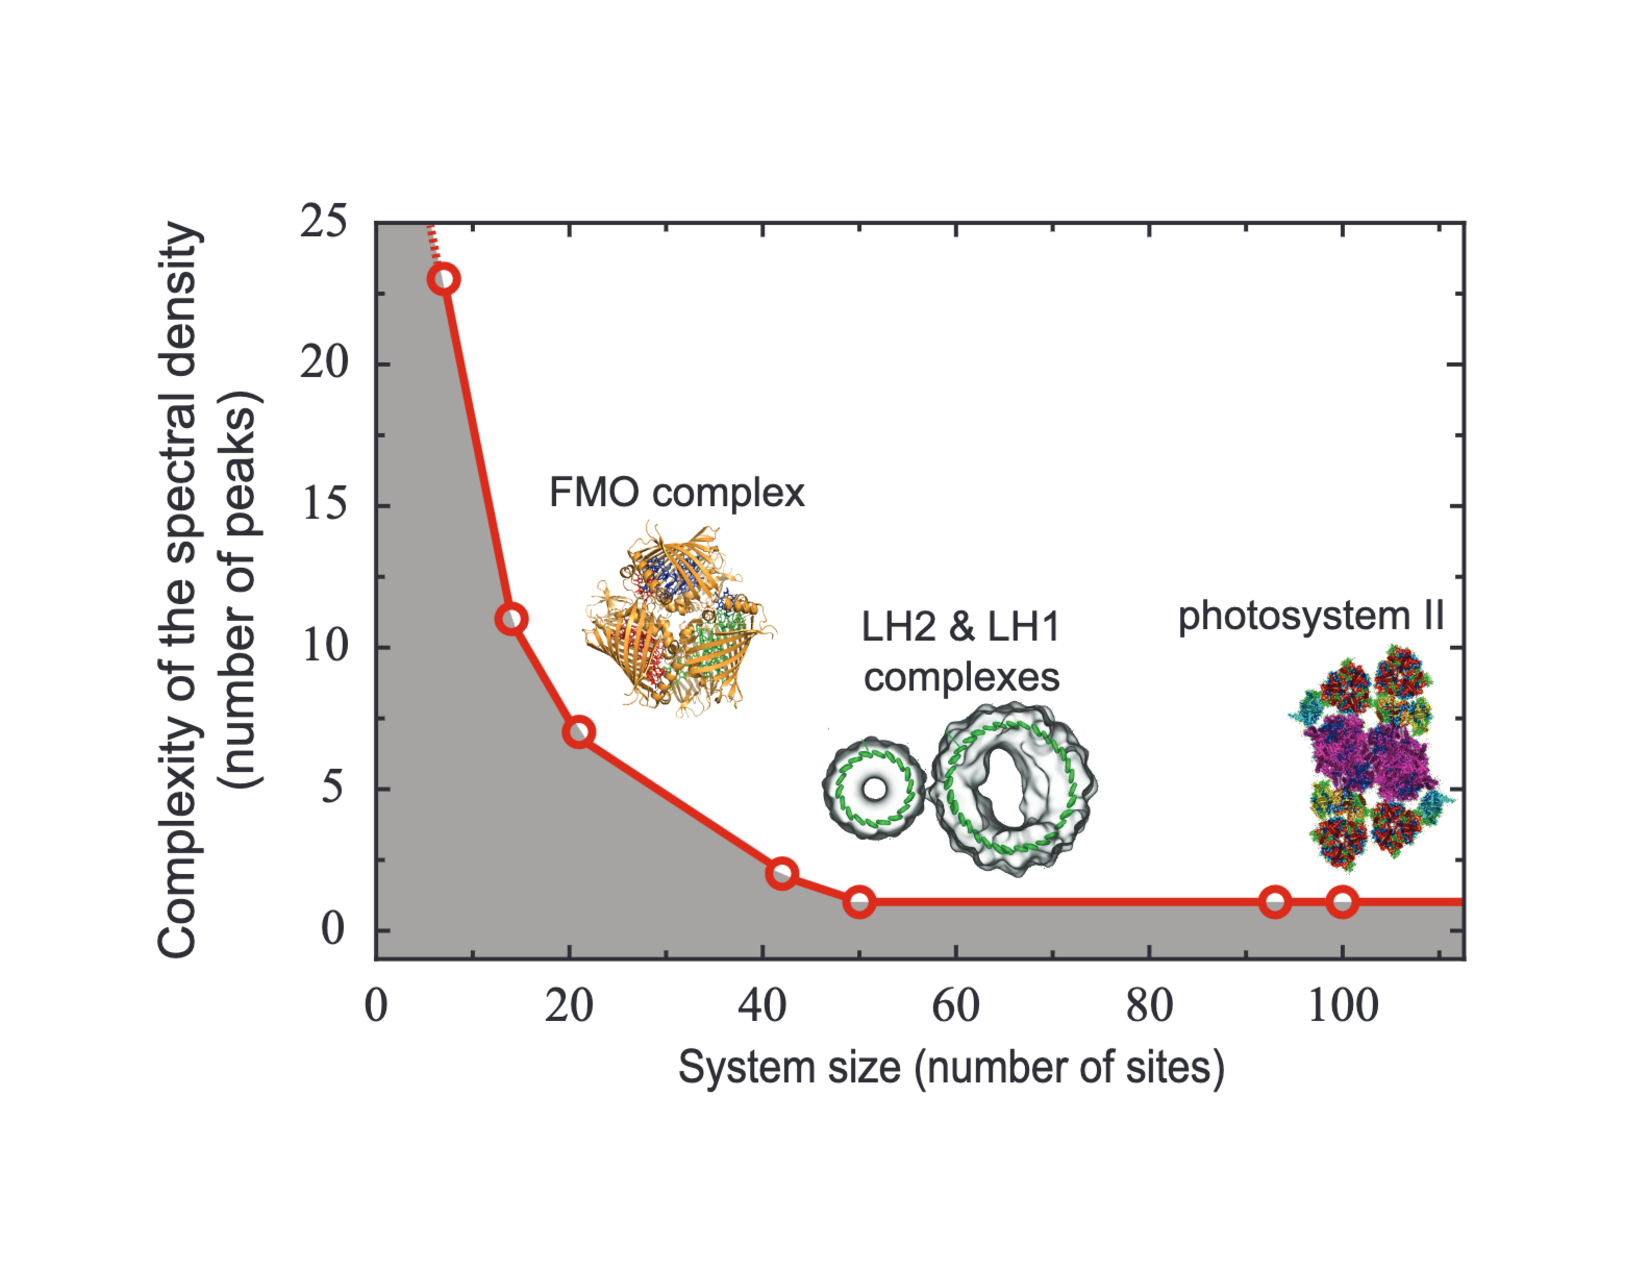
\includegraphics[width=\columnwidth]{Frenkel_exciton_Hamiltonians.pdf}
    \caption{The shaded region in the graph illustrates the estimated sizes of treatable systems when simulating Frenkel exciton Hamiltonians using current classical supercomputing resources.  Three photosynthetic systems are presented: the Fenna-Matthews-Olson complex of Green-Sulfur Bacteria, the Light Harvesting I and II complexes of Purple Bacteria, and Photosystem II of higher plants. The simulation was conducted utilizing the hierarchical equations of motion approach on 64 AMD Opteron cores, utilizing a total of 250 GB of RAM. Image from~\cite{Mostame2016}.}
    \label{fig:Frenkel}
\end{figure}

\subsubsection{Coarse-grained simulations}


The commercialization of new, advanced materials is often a cost-, time-, and labor-intensive process.  Typical times to bring a new material to market are on the order of 10-20 years from initial research to first use \cite{national2011materials}.
The long, expensive commercialization process is partially due to the experimental nature of materials development, e.g., many material samples must be physically prepared and then evaluated.  Challenges in the process include the sample preparation, which for new materials has a steep learning curve, with many iterations of learning required to identify the best methods to create high-quality samples for evaluation.  The precursors and by-products for sample preparation may be expensive, hard to obtain, and/or unsafe, thus requiring specialized equipment to handle.  Further, evaluation of the samples may be laborious with many data points to be taken under carefully controlled conditions.  Finally, more often than not, once a sample is finally prepared and evaluated, the conclusion is that the material does not meet the desired specifications, and the entire process must be repeated for a different material candidate.

The materials commercialization process may be accelerated by conducting material exploration computationally.  New materials may be evaluated quickly and efficiently by virtually modeling a material and predicting its properties.  The role of experimentation is moved from exploration to confirmation of the computational results. 

In computational materials discovery, the process often has two steps.  The first identifies or generates material candidates, which may be done, for example, with machine learning methods.  In the second step, the material candidates are filtered by computationally predicting their material properties.  Methods to compute material properties are discussed here.

One type of material property in demand is those that are both light and strong. The main modeling for these concerns two main areas. The first is materials discovery, in which computation is used to test predicted materials' stability. This includes stability against spontaneous transition to alternative undesirable phases with the application of small amounts of pressure or temperature change; or indeed stability against phase separation, in which constituent atoms cluster together and do not form compounds or layers as desired. The computational tests for this include perturbing atomic positions and seeing minute energy changes in order to infer reaction barriers. These are DFT calculations using often nudged elastic band techniques. Additional tests are done by calculating the phonon spectra. A state-of-the-art set of such tests appears in \cite{long2023two}, pages 6-8.

   The second main area of modeling for advanced materials is defect studies: crack propagation and corrosion are two key areas. Both of these defects can be either across a surface in the form of failure of protective coatings and surface cracks; or deep into a surface, whether a crack or deep pit corrosion. Failure of mechanical properties occurs on all length scales, starting at the atomic and spreading to macroscopic, visible effects on the scale or centimeters or longer. For this, the main modeling approach is a type of embedding theory as introduced above. The essence of embedding techniques is a set of calculations that are done at much higher accuracy, usually at the cost of both time and resources, in a key important region chosen as the active space. The results of the embedding calculations then need to be matched to those done at a coarser level, a challenging task to do well, and which difficulty depends to some degree on the type of embedding done, see the paragraph below. For example, if the type of embedding is by calculating quantum wave functions in the active space, connecting to classical more macroscopic descriptions of phonon and other vibrational levels can be a very challenging task. However, if instead the active space consists of precise calculations of atomic positions at zero temperature, then these can be connected to those at finite temperature by a process of ramping up vibrations, and this can work quite well. When the defect to be modeled, such as a crack, occurs at multiple length scales, then each scale working up from the smallest to the largest can be considered the embedded active space of the one that comes at a larger scale, and matching must be done at each stage. This is termed multi-scale quantum embedding. 
   
   Both for crack propagation and defect modeling such as corrosion of the key material or failure of a coating, often first-principles molecular dynamics is also used, with DFT used to calculate the forces and energies. These calculations are used both to test the matching at the different scales and also as a study tool in itself, to try to infer mechanisms for materials failure. With a crack, the action can spread very quickly from the atomic to the macroscopic, if forces are strong enough, and MD is key for measures of the speed of such scale transitions. For other kinds of defects such as wear and corrosion, processes typically happen on a much slower time scale, and deeper calculations can be done at the atomic level to study the origins of the failure. However, in almost all cases, these, too, are done with quantum embedding methods of detailed fully quantum calculations, often extending to full-configurational chemistry, for the active regions.

   Other types of material challenges are in handling creep, a slow deformation when a material is exposed to long-term stress (pressure, force, twist). These types of slower macroscopic changes are usually treated with differential equations, which have optimal algorithms in quantum computing, particularly if the problem can be linearized. Additional observables such as Young's modulus and Poisson's ratio measure the properties of materials and can reveal defects if the material is not up to the expected level. Methods to compute these properties are also on a macroscopic scale and use both differential and integral equations. 

   When materials are exposed to magnetic or electrical fields, we term these open quantum problems. Systems in magnetic or electrical fields are known as driven systems, and those at finite temperatures as dissipative systems. Thus one can have a driven, dissipative system. These types of systems are usually handled with lattice models, as discussed in a previous Subsection.

\subsubsection{An example use case: quantum metamaterials}

The above use cases show how quantum and classical computing can effectively work together to answer key questions in materials design.  As noted in our criteria, such modeling must be relevant to real-world problems, challenging to simulate classically, include feasibly solvable sub-problems on quantum computers, and potentially involve classical HPC and quantum computers in concert.  The overall evolution of simulation in materials discovery generally follows the three phases of phenomenological simulation for insight, property prediction for candidate screening, and finally direct optimization of materials for target properties.  To illustrate this further, we explore an example use case of metamaterials in more detail.

The design of metamaterials, characterized by their unique properties like negative refractive index and selective spectral reflection, holds immense promise for diverse real-world applications \cite{doi:10.1126/science.1096796,10.1038/natrevmats.2016.1,10.1038/natrevmats.2017.66,10.1038/s41928-019-0257-7}. These artificially structured materials, functioning at sub-wavelength scales, offer a novel path to enhance the performance of conventional electronic devices. This improvement, in turn, has the potential to revolutionize energy-saving in fields such as thermophotovoltaics, heating, ventilation, and air conditioning systems. Consequently, the pursuit of optimal metamaterial designs has become an area of intense research interest.

\begin{figure}
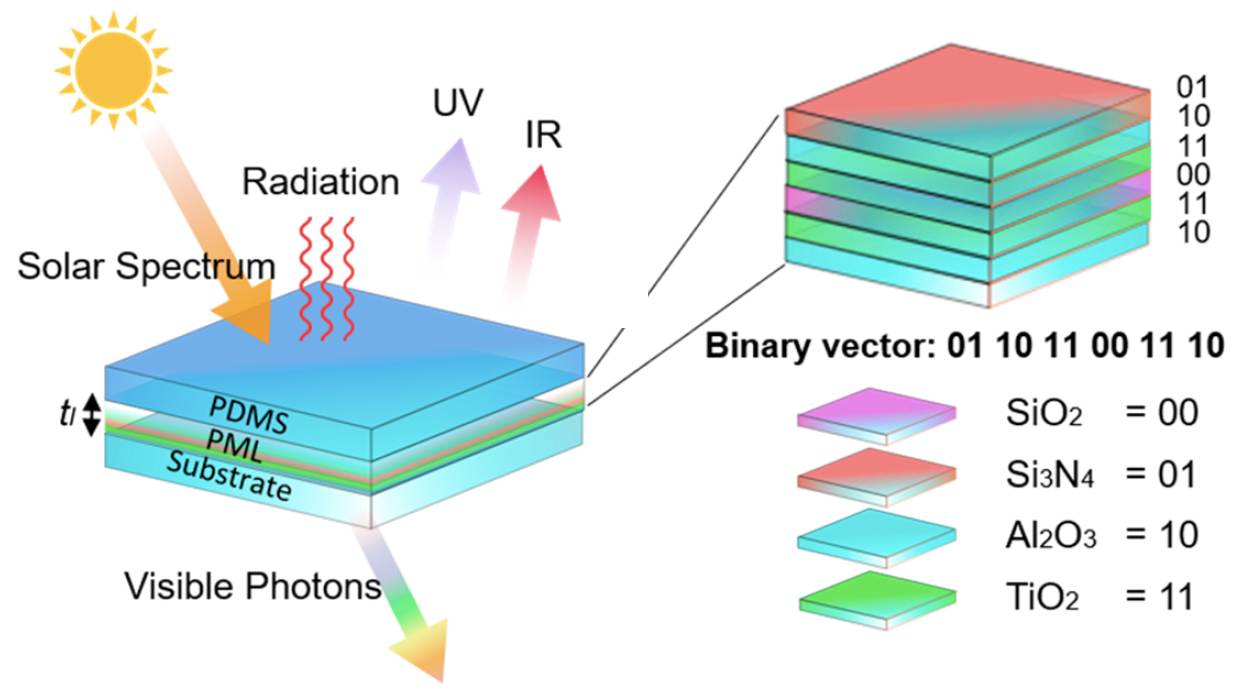
\includegraphics[width=\columnwidth]{groups/2._Use_case_discovery/metamaterial-fig.png}
\caption{The schematic structure of the planar multi-layer in the transparent radiative cooling metamaterial that can be mapped into a binary vector (from \cite{10.1021/acsenergylett.2c01969}).}
\label{fig:metamaterial}
\end{figure}

The properties of metamaterials hinge not only on their inherent material characteristics but also on their geometric parameters. Therefore, determining the ideal geometrical parameters is fundamental to achieving high-performance metamaterials. However, the challenge arises from the multi-dimensional nature of these parameters, creating vast, non-convex design spaces. As such, finding the optimal metamaterial structures through intuition, trial-and-error, exhaustive searches, or random approaches becomes a complex and laborious task.

This leads to essential questions in metamaterial design:
How can we identify high-performance metamaterials that are close to the global optimal design?
How can we optimally design metamaterials with complex geometric parameters that lead to significantly large design spaces?
To address these questions, a novel strategy is proposed - an active learning algorithm that harnesses the power of machine learning, quantum computing, and HPC to efficiently design metamaterials, even in cases with complex target properties and expansive search spaces. Metamaterials, often consisting of discretized design concepts, necessitate effective solutions for combinatorial optimization problems. Quantum computing, exploiting the unique principles of quantum physics like superposition, entanglement, and tunneling, offers exponential computational speedup over classical computing \cite{10.1038/nphys2900}.

To solve optimization problems using quantum computing processors, an objective function is formulated as a Hamiltonian, describing the relationship between metamaterial states and their properties. Factorization machine, a supervised machine learning model, can effectively capture the relationship between input variables and output values, providing model parameters such as bias, linear terms, and quadratic terms. These parameters can be directly utilized to construct a Hamiltonian matrix \cite{5694074}. Consequently, an iterative algorithm that combines factorization machines \cite{PhysRevResearch.2.013319} and quantum computing can efficiently discover optimal metamaterial designs.

Despite the efficiency of quantum computing in solving Hamiltonian objective functions, current quantum devices have a limited number of qubits. Thus, their utility for numerical simulations is restricted. Parallel computing, particularly HPC, holds the potential to provide substantial acceleration for such tasks. Therefore, the integration of machine learning, quantum computing, and HPC emerges as a powerful approach for the efficient design of complex metamaterials.
One more question emerges: How can continuous variables be optimized using a quantum computing-based algorithm, which typically returns binary variables? To address this limitation, another quantum computing-based algorithm is proposed \cite{PhysRevResearch.4.023062}, capable of simultaneously optimizing discrete and continuous spaces, making it a more versatile tool in metamaterial design.
